\subsection{Tenants}
\label{sec:application:building_the_model:tenants}

The eighth step introduces another class type. This time, the $.\type{Tenant}$ type is introduced to enrich the model and graphs even further. \cref{subsec:library_of_transformations:type_level_transformations:regular_classes} is used to introduce the class type, while on the instance level, \cref{subsec:library_of_transformations:instance_level_transformations:plain_objects} is used to introduce the house objects.

The $name$ of the new tenant type is $.\type{Tenant}$. Furthermore, 5 tenant objects are introduced, $objects = \{Tenant1, Tenant2, Tenant3, Tenant4, Tenant5\}$. Furthermore, we assume that the object identifiers are equal to the internal node id, so $fid(Tenant1) = Tenant1$ and $fid(Tenant2) = Tenant2$, etc. The following model is obtained:

\LTXtable{\textwidth}{tex/06_application/02_building_the_model/tables/08_tenants.tex}

\begin{figure}[p]
    \centering
    \begin{subfigure}{0.98\textwidth}
        \centering
        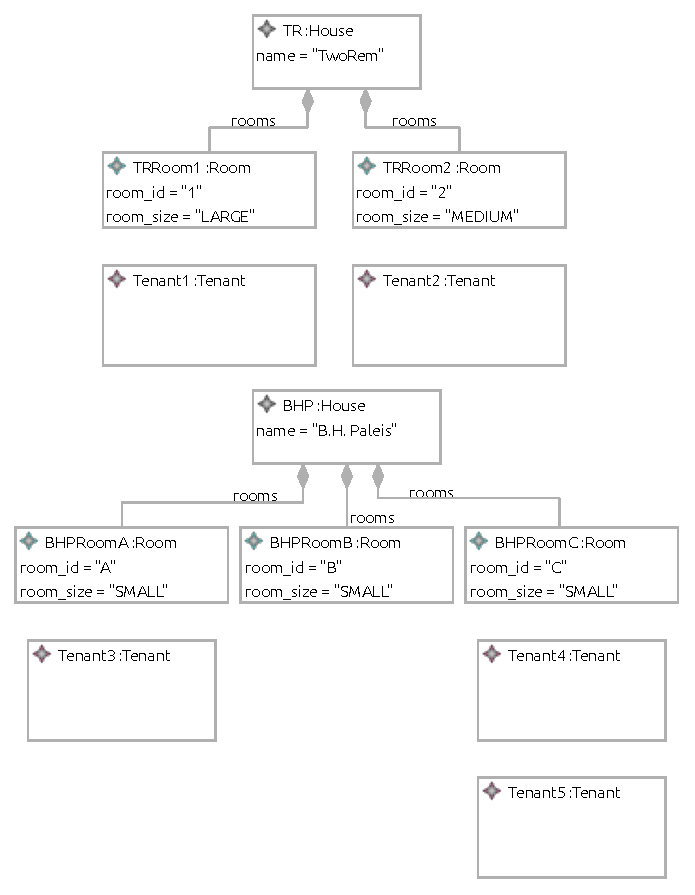
\includegraphics{images/06_application/instance_model/step08.pdf}
        \caption{Instance Model $Im_8$}
        \label{fig:application:building_the_model:tenants:ecore:instance_model}
    \end{subfigure}
    \\
    \begin{subfigure}{0.98\textwidth}
        \centering
        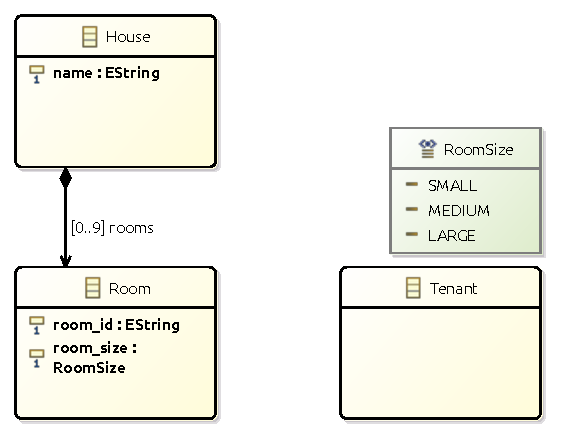
\includegraphics{images/06_application/type_model/step08.pdf}
        \caption{Type Model $Tm_8$}
        \label{fig:application:building_the_model:tenants:ecore:type_model}
    \end{subfigure}
    \caption{The Ecore model after step 8}
    \label{fig:application:building_the_model:tenants:ecore}
\end{figure}

\begin{figure}[p]
    \centering
    \begin{subfigure}{0.98\textwidth}
        \centering
        % To use this figure in your LaTeX document
% import the package groove/resources/groove2tikz.sty
%
\begin{tikzpicture}[scale=\tikzscale,name prefix=step08-]
\node[type_node] (n0) at (0.740, -0.400) {\ml{\textbf{House}\\name: \textbf{string}}};
\node[type_node] (n1) at (0.730, -1.585) {\ml{\textbf{Room}\\room\_id: \textbf{string}}};
\node[type_node] (n2) at (2.380, -0.560) {\ml{\textbf{RoomSize}\\\textit{LARGE}\\\textit{MEDIUM}\\\textit{SMALL}}};
\node[type_node] (n3) at (2.500, -1.590) {\ml{\textbf{Tenant}}};

\path[basic_edge, composite](n0.south -| 0.730, -1.585) -- node[lab] {\ml{rooms}} (n1) ;
\path[basic_edge] (n1)  -- node[lab] {\ml{room\_size}} (n2) ;
\end{tikzpicture}

        \caption{Instance Graph $IG_8$}
        \label{fig:application:building_the_model:tenants:groove:instance_graph}
    \end{subfigure}
    \\
    \begin{subfigure}{0.98\textwidth}
        \centering
        % To use this figure in your LaTeX document
% import the package groove/resources/groove2tikz.sty
%
\begin{tikzpicture}[scale=\tikzscale,name prefix=step08-]
\node[type_node] (n0) at (0.740, -0.400) {\ml{\textbf{House}\\name: \textbf{string}}};
\node[type_node] (n1) at (0.730, -1.585) {\ml{\textbf{Room}\\room\_id: \textbf{string}}};
\node[type_node] (n2) at (2.380, -0.560) {\ml{\textbf{RoomSize}\\\textit{LARGE}\\\textit{MEDIUM}\\\textit{SMALL}}};
\node[type_node] (n3) at (2.500, -1.590) {\ml{\textbf{Tenant}}};

\path[basic_edge, composite](n0.south -| 0.730, -1.585) -- node[lab] {\ml{rooms}} (n1) ;
\path[basic_edge] (n1)  -- node[lab] {\ml{room\_size}} (n2) ;
\end{tikzpicture}

        \caption{Type Graph $TG_8$}
        \label{fig:application:building_the_model:tenants:groove:type_graph}
    \end{subfigure}
    \caption{The GROOVE graphs after step 8}
    \label{fig:application:building_the_model:tenants:groove}
\end{figure}

A visual representation of $Tm_8$ and $Im_8$ can be found in \cref{fig:application:building_the_model:tenants:ecore}. Similarly, a visual representation of $TG_8$ and $IG_8$ can be found in \cref{fig:application:building_the_model:tenants:groove}. Please note that because of the definitions of $f_8(Im_8)$ and $f'_8(IG_8)$, we have that $f_8(Im_8) = IG_8$ and $f'_8(IG_8) = Im_8$. Furthermore, $f_8(Im_8)$ and $f'_8(IG_8)$ are valid mapping functions themselves, such that they can be combined with another mapping function in the next step.

The introduction of the tenant class shows that models can be extended if there is already much information in the model. Introducing types can be done at any moment, so there is no need to introduce all types at the beginning. In that sense, the transformation framework presented by this thesis is not deterministic; there are multiple ways to encode the same model.

\afterpage{\FloatBarrier}